\subsubsection{Concept}
% The concept of the cyborg is inspired by similar efforts such as
% \cite{li_application_2015} and \cite{warwick paper}.
% Fig \ref{fig:cyborg_idea} shows the basic premise: An in-vitro neuron culture will be used to
% control a robot in a closed loop system, making the robot an actual cyborg.
The main challenge creating a cyborg is harnessing and applying the
computational power of neurons to enhance the capability of the robot, showing
that the neurons are actually doing something useful.
As previously discussed the function of neural networks are vastly complex,
attempting to fully understand the complex interplay of chemical and electrical
signals is intractable.
Therefore, in order to interface with the neural network we employ the mindset
of reservoir computing.
From this perspective we can reduce the complexity of the task significantly.
The first benefit is that we can choose to focus on only electrical signals,
which vastly reduces the search space at a minimal information loss cost. 
Secondly we have now avoided having to explicitly train the neurons towards
performing their task, we now view them as a reservoir for dynamics which
responds to stimuli, leaving the task of translating this response into useful
actions.
In \ref{fig:cyborg_idea} this approach is visualized:
A neural network is grown in a \textit{micro electrode array} which allows
interfacing with a neuron culture by measuring and inducing voltages on an array
of electrodes which the neurons grow around.
This partial view of the complete system is interpreted by an artificial
neural network which outputs commands to a robot.
Similarly feedback is provided to the neural network from the sensors of the
robot which is translated into electrical stimuli requests by a feedback processor.
\begin{figure}[h!]
    %\centering
    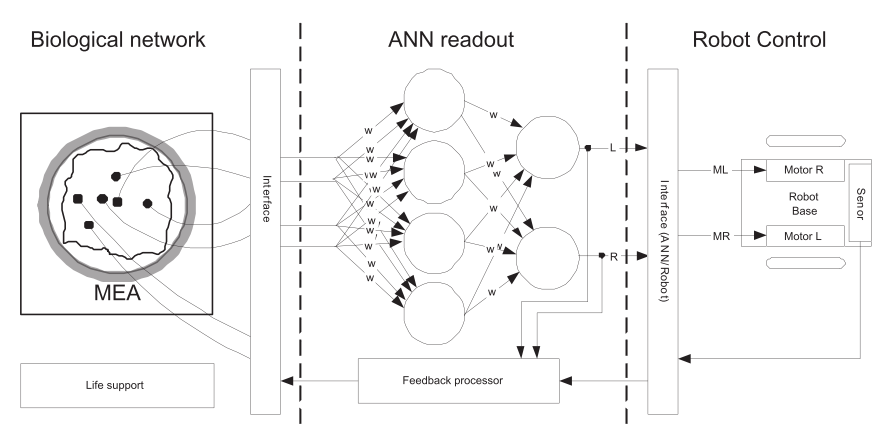
\includegraphics[width=\linewidth]{images/cyborg_overview.png}
    \caption{The gist of it..}
    \label{fig:cyborg_idea}
\end{figure}
\subsubsection{Platform}
Providing an interface between neurons and a computer is an important first
step, however it is highly impractical to move the neural cultures outside of
the laboratory.
The practical solution is quite thought provoking\footnote{For brevity the
  philosophical implications is left as an exercise to the reader.},
by using a TCP/IP network protocol the neuron culture may be interfaced with any
robot or simulator without leaving the laboratory. 
Similar network architectures have been implemented, in
\cite{li_application_2015} a neuron culture is used to control a simple wall
avoiding robot, \#\# something about the shortcomings of this paper \#\#.
% The architecture described in this paper is a refinement of the neuro-robot
% architecture used in \cite{li_application_2015}.
% In \cite{li_application_2015} a system for working specifically with MEAs
% containing dissociated neurons is described with a TCP/IP connection to a slave
% PC controlling a robot being the main selling point. Our model is a
% generalization of \cite{li_application_2015} designed for reservoir computing,
% where the neuron-culture is just one of many possible reservoirs.
% It should be noted that our architecture does not require experiments to be
% posed in the context of reservoir computing. (not too happy with the words here,
% make them betterer. Also something about the possibility of multiple implementations)
\subsubsection{Growing NIV}

\subsubsection{A First Test}
\begin{figure}[h!]
    %\centering
    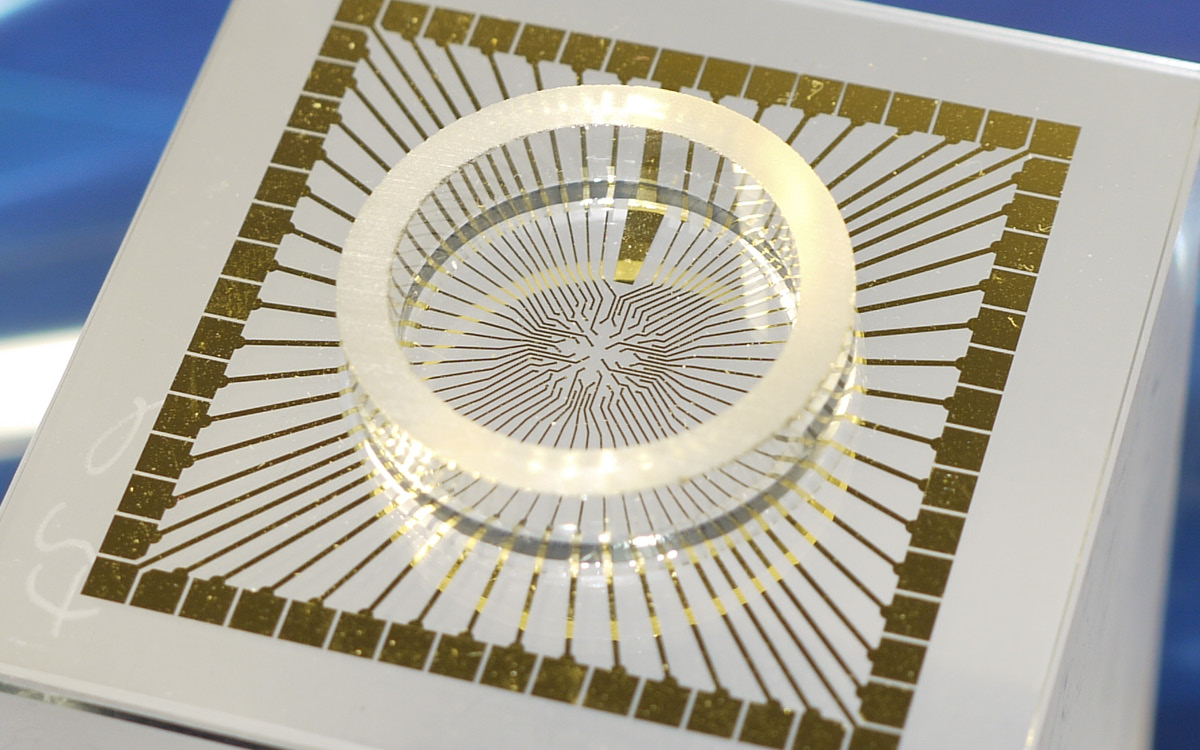
\includegraphics[width=\linewidth]{images/MEA.jpg}
    \caption{A generic MEA}
    \label{fig:generic_MEA}
\end{figure}

\begin{figure}[h!]
    %\centering
    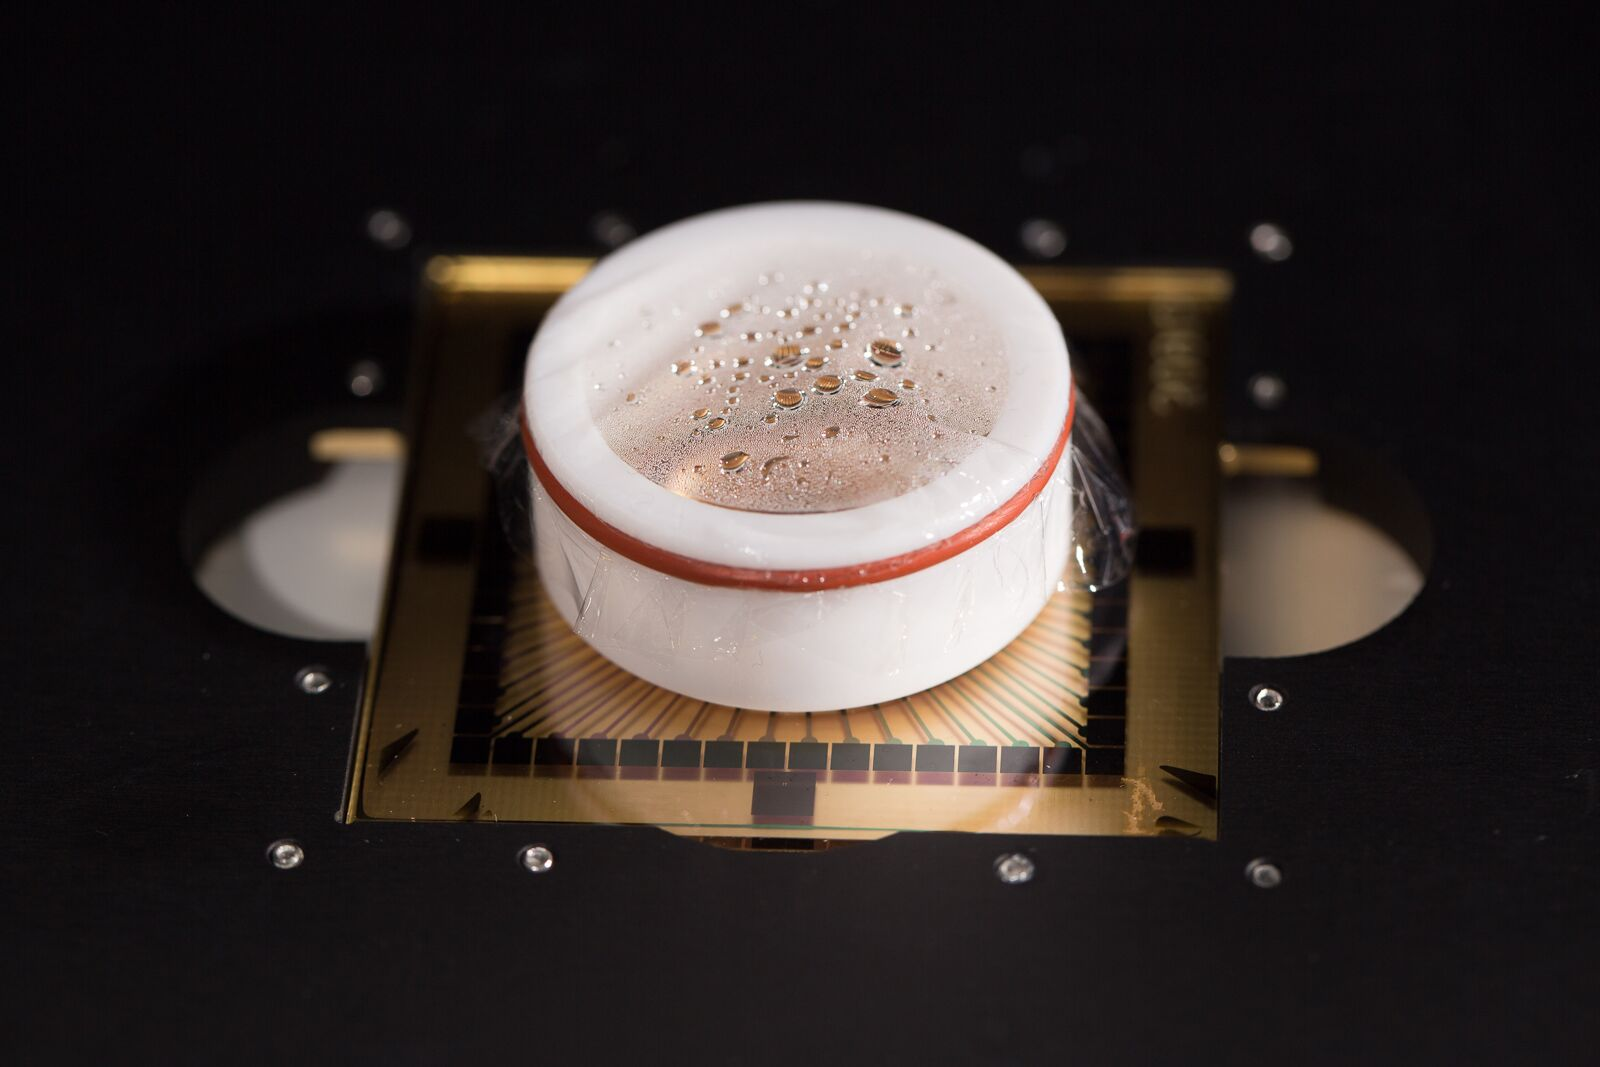
\includegraphics[width=\linewidth]{images/st-olavs-mea.jpg}
    \caption{A MEA with a live culture, photographed by Kai}
    \label{fig:st_olav_MEA}
\end{figure}
\begin{figure}[h!]
    %\centering
    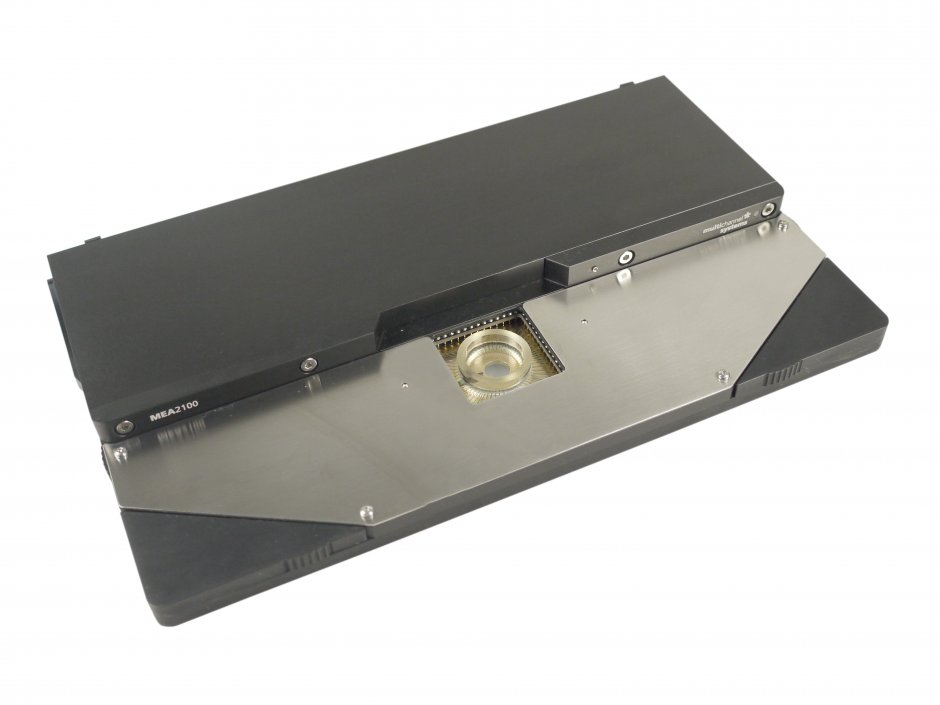
\includegraphics[width=\linewidth]{images/MEA2100-HS60.jpg}
    \caption{The headstage}
    \label{fig:headstage}
\end{figure}
\begin{figure}[h!]
    %\centering
    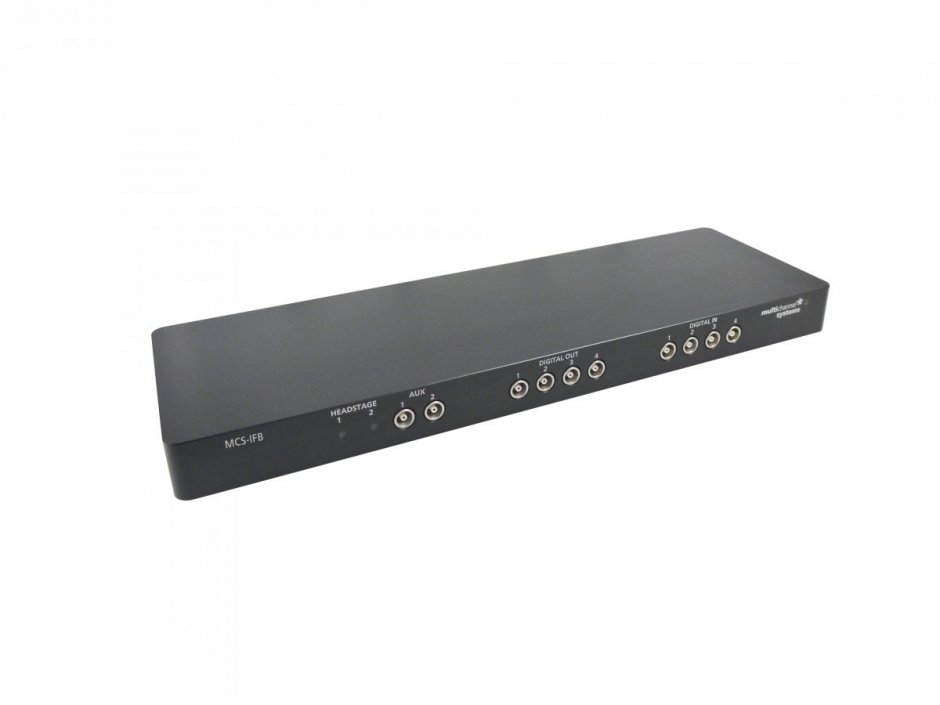
\includegraphics[width=\linewidth]{images/MCS-IFB.jpg}
    \caption{The MCS interface board}
    \label{fig:neuron_anatomy}
\end{figure}
%%% Local Variables:
%%% mode: latex
%%% TeX-master: "../main"
%%% End:
